% Native vector figures for Experiment 13 unified flagship Rev. 5 candidate.
% Grayscale, APS two-column safe.

\newcommand{\RevFigStages}{%
\begin{figure}[tbp]
\centering
\resizebox{\columnwidth}{!}{%
\begin{tikzpicture}[>=Latex,every node/.style={font=\sffamily\small}]
\tikzset{stage/.style={draw,rounded corners=1.5pt,minimum width=2.45cm,minimum height=1.08cm,align=center,inner sep=4pt}}
\node[stage] (task) at (0,0) {task / signal\\$\mathcal H_{\rm task}$};
\node[stage] (exc) at (3.18,0) {optical excitation\\$\mathcal H_{\rm exc}$};
\node[stage] (int) at (6.36,0) {internal dynamics\\$\mathcal H_{\rm int}$};
\node[stage] (term) at (9.54,0) {terminal readout\\$\mathcal H_{\rm term}$};
\draw[->,line width=.8pt] (task)--node[above,font=\scriptsize]{$M_{\rm opt}$}(exc);
\draw[->,line width=.8pt] (exc)--node[above,font=\scriptsize]{$M_{\rm dyn}$}(int);
\draw[->,line width=.8pt] (int)--node[above,font=\scriptsize]{$M_{\rm ro}(\omega)$}(term);
\node[font=\scriptsize,align=center] at (3.18,-1.05) {stage-specific inference: properties do not transfer\\without the intervening physical map};
\draw[decorate,decoration={brace,mirror,amplitude=4pt},line width=.6pt] (-1.15,-.62)--(10.70,-.62);
\node[font=\scriptsize,align=center] at (1.55,1.08) {capacity};
\node[font=\scriptsize,align=center] at (4.77,1.08) {selectivity};
\node[font=\scriptsize,align=center] at (8.00,1.08) {observability};
\end{tikzpicture}}
\caption{Detector inference is stage-specific. Optical coupling, internal dynamics, and terminal readout are different physical maps. A capacity, singular-value distribution, or null space at one stage cannot be transferred to another without the intervening dynamics.}
\label{fig:stages}
\end{figure}%
}

\newcommand{\RevFigTheorem}{%
\begin{figure}[tbp]
\centering
\resizebox{0.92\columnwidth}{!}{%
\begin{tikzpicture}[>=Latex,every node/.style={font=\sffamily\small}]
\tikzset{box/.style={draw,rounded corners=1.5pt,minimum width=4.0cm,minimum height=1.0cm,align=center,inner sep=4pt}}
\node[box] (sig) at (0,2.85) {$\sigma_1^{\rm cross}(\omega)$\\selected direct response};
\node[box] (strength) at (0,1.25) {$\mathcal L_{\mathcal B}\le\mathcal R_{\mathcal B}$\\Fermi/Kubo strength step};
\node[box,minimum width=3.4cm] (cap) at (5.0,1.25) {$(v_{\mathcal B}^{\rm cap})^2$\\exact-shell capacity};
\node[box,minimum width=5.0cm] (pop) at (2.5,-0.55) {$n_e+n_h\ge n_{\mathcal B}^{\rm act}\ge\mathcal L_{\mathcal B}/(v_{\mathcal B}^{\rm cap})^2$};
\draw[->,line width=.8pt] (sig)--node[right,font=\scriptsize]{Fermi + Kubo}(strength);
\draw[->,line width=.8pt] (strength)--(pop);
\draw[->,line width=.8pt] (cap)--(pop);
\end{tikzpicture}}
\caption{Logical structure of the principal semiconductor theorem. Fermi statistics convert selected conductivity into a lower optical-strength functional; the independently declared exact-shell velocity capacity then converts that strength into a lower bound on active thermal endpoint population.}
\label{fig:theorem-flow}
\end{figure}%
}

\newcommand{\RevFigGeometry}{%
\begin{figure}[tbp]
\centering
\resizebox{\columnwidth}{!}{%
\begin{tikzpicture}[>=Latex,every node/.style={font=\sffamily\small}]
\tikzset{fbox/.style={draw,rounded corners=1.5pt,minimum width=2.25cm,minimum height=1.05cm,align=center,inner sep=4pt}}
\node[fbox] (support) at (0,0) {support coverage\\$n_{\mathcal B}^{\rm act}/n_{\rm ref}$};
\node[fbox] (fermi) at (2.80,0) {Fermi/Kubo\\$\eta_F$};
\node[fbox] (shell) at (5.60,0) {shell / global\\$c_a$};
\node[fbox] (within) at (8.40,0) {within shell\\$1/\mathcal S_a^{\rm act}$};
\draw[->,line width=.8pt] (support)--(fermi);
\draw[->,line width=.8pt] (fermi)--(shell);
\draw[->,line width=.8pt] (shell)--(within);
\node[draw,rounded corners=1.5pt,align=center,minimum width=8.1cm,minimum height=1.05cm] at (4.20,-1.70)
{$\displaystyle \frac{n_{\rm bound}}{n_{\rm ref}}=\frac{n_{\mathcal B}^{\rm act}}{n_{\rm ref}}\,\eta_F\,\sum_a w_a^{\rm act}\frac{c_a}{\mathcal S_a^{\rm act}}$};
\node[font=\scriptsize,align=center] at (4.20,1.05) {four identifiable places where inverse population information can be lost};
\end{tikzpicture}}
\caption{Full population-bound tightness hierarchy. The bound/reference ratio separates incomplete selected support, Fermi/Kubo asymmetry, shell-to-global capacity mismatch, and within-shell response selectivity. This decomposition is the physically informative content behind the fixed-map capacity normalization.}
\label{fig:geometry}
\end{figure}%
}

\newcommand{\RevFigHgCdTe}{%
\begin{figure}[tbp]
\centering
\resizebox{\columnwidth}{!}{%
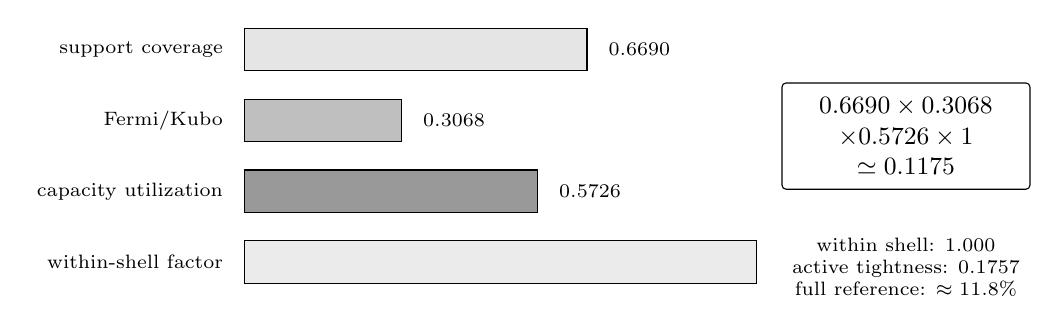
\begin{tikzpicture}[every node/.style={font=\sffamily\small}]
\def\W{6.5}
\node[anchor=east,font=\scriptsize] at (0,3.35) {support coverage};
\node[anchor=east,font=\scriptsize] at (0,2.45) {Fermi/Kubo};
\node[anchor=east,font=\scriptsize] at (0,1.55) {capacity utilization};
\node[anchor=east,font=\scriptsize] at (0,.65) {within-shell factor};
\draw[fill=black!10,draw=black] (.15,3.08) rectangle ({.15+\W*.66897},3.62);
\draw[fill=black!25,draw=black] (.15,2.18) rectangle ({.15+\W*.30684},2.72);
\draw[fill=black!40,draw=black] (.15,1.28) rectangle ({.15+\W*.57262},1.82);
\draw[fill=black!08,draw=black] (.15,.38) rectangle ({.15+\W},.92);
\node[anchor=west,font=\bfseries\scriptsize] at ({.30+\W*.66897},3.35) {$0.6690$};
\node[anchor=west,font=\bfseries\scriptsize] at ({.30+\W*.30684},2.45) {$0.3068$};
\node[anchor=west,font=\bfseries\scriptsize] at ({.30+\W*.57262},1.55) {$0.5726$};
\node[draw,rounded corners=1.5pt,align=center,minimum width=3.15cm,minimum height=1.35cm] at (8.55,2.25)
{$0.6690\times0.3068$\\$\times0.5726\times1$\\$\simeq0.1175$};
\node[font=\scriptsize,align=center] at (8.55,.58) {within shell: $1.000$\\active tightness: $0.1757$\\full reference: $\approx11.8\%$};
\end{tikzpicture}}
\caption{HgCdTe closure of the full hierarchy for the broad 300-K window. The selected active population covers about $0.669$ of the reference population; the Fermi/Kubo and capacity factors are $0.3068$ and $0.5726$; and the single-parent-doublet sectors have no additional within-shell penalty in the BIA-neglecting validation.}
\label{fig:hgcdte}
\end{figure}%
}

\newcommand{\RevFigRecycling}{%
\begin{figure}[tbp]
\centering
\resizebox{\columnwidth}{!}{%
\begin{tikzpicture}[>=Latex,every node/.style={font=\sffamily\small}]
\node[font=\bfseries\small] at (2.45,3.20) {(a) ideal final-sink counting};
\node[draw,minimum width=.95cm,minimum height=.70cm] (A1) at (.65,1.85) {A};
\node[draw,minimum width=.95cm,minimum height=.70cm] (B1) at (4.25,1.85) {B};
\draw[->,line width=.8pt] (A1)--node[above,font=\scriptsize]{recycle}(B1);
\node[font=\scriptsize,align=center] at (.65,.65) {source channel\\$H_A^{\rm end}=0$};
\node[font=\scriptsize,align=center] at (4.25,.65) {one final sink\\$H_B^{\rm end}\neq0$};
\draw[densely dashed] (A1.south)--(.65,1.03);
\draw[->] (B1.south)--(4.25,1.03);

\node[font=\bfseries\small] at (8.15,3.20) {(b) finite-transit Ramo readout};
\node[draw,minimum width=.95cm,minimum height=.70cm] (A2) at (6.10,1.85) {A};
\node[draw,minimum width=.95cm,minimum height=.70cm] (B2) at (10.10,1.85) {B};
\draw[->,line width=.8pt] (A2)--node[above,font=\scriptsize]{recycle / transit}(B2);
\draw[->] (5.95,.20)--(9.20,.20) node[right,font=\scriptsize]{$t$};
\draw[->] (6.20,-.55)--(6.20,1.03) node[above,font=\scriptsize]{$i_A$};
\draw[line width=.85pt] plot[smooth] coordinates {(6.20,.20)(6.55,.78)(6.95,.45)(7.35,-.25)(7.78,-.05)(8.28,.20)};
\node[font=\scriptsize,align=center] at (9.52,.08) {$\int i_A dt=0$\\but $H_A(\omega\ne0)$ can survive};
\node[font=\scriptsize,align=center] at (8.15,-.72) {single-lineage source null can be lifted at finite frequency};
\end{tikzpicture}}
\caption{Readout-dependent observability of one conservative A-to-B recycling lineage. Exclusive final-sink counting can place the lineage in the source-channel null. Finite-transit Shockley--Ramo current can restore source-channel finite-frequency support even though the internally created and recombined segment has zero integrated induced charge.}
\label{fig:recycling}
\end{figure}%
}
